\section{Theorie}
\label{sec:Theorie}

\subsection{Einleitung}

Im folgenden Experiment werden diverse Schaltungen mit Operationsverstärkern
aufgebaut und ausgemessen um ein besseres Verständnis von diesen zu erhalten.
Dazu werden zunächst einige theoretische Grundlagen in den folgenden Abschnitten
bereitgestellt.

\subsection{Funktionsweise und Kenngrößen eines Operationsverstärkers}

Ein Operationsverstärker ist im Wesentlichen ein Differenzverstärker, der in der Lage ist, eine Eingangsspannungsdifferenz
mit Hilfe zweier Betriebsspannungen unterschiedlichen Vorzeichens zu verstärken.
Die dafür notwendige Beschaltung ist in Abbildung \ref{fig:OPVGrund} schematisch dargestellt.

\begin{figure}
  \centering
  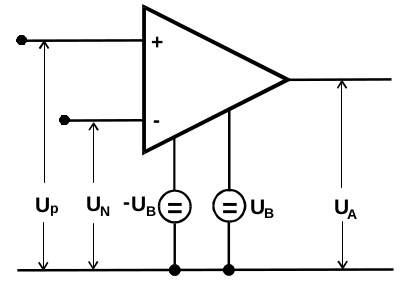
\includegraphics[height=5cm]{ImmerDieseNorweger/OPVGrund.png}
  \caption{Schematische Darstellung der grundlegenden Beschaltung eines Operationsverstärkers \cite{anleitung}.}
  \label{fig:OPVGrund}
\end{figure}

Die Spannung $U_\text{p}$, die am sogenannten nicht-invertierenden Eingang $(+)$ anliegt, geht positiv
in die Ausgangsspannung $U_\text{A}$ ein und ist entsprechend mit ihr in Phase, während die Spannung $U_\text{N}$,
welche am invertierenden Eingang $(-)$ anliegt, abgezogen wird und entsprechend gegenphasig zur Ausgangsspannung ist.
Innerhalb des sogenannten Aussteuerungsbereichs, welcher gemäß
\begin{align}
  -U_\text{B} < U_\text{A} < U_\text{B},
\end{align}
durch die Betriebsspannungen $U_\text{B}$ gegeben ist, gilt für die Ausgangsspannung $U_\text{A}$ ein linearer Zusammenhang
\begin{align}
  U_\text{A} = V \left( U_\text{p} - U_\text{N} \right),
\end{align}
wobei $V$ der Verstärkungsfaktor ist. Außerhalb dieses Bereichs geht $U_\text{A}$ in eine
Sättigung und nähert sich den Werten $\pm U_\text{B}$ an.
Die soeben beschriebene Kennlinie eines Operationsverstärkers ist in Abbildung \ref{fig:kennlinieOPV}
noch einmal skizziert.

\begin{figure}
  \centering
  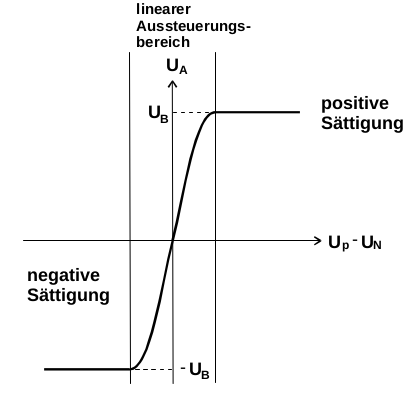
\includegraphics[height=7cm]{ImmerDieseNorweger/kennlinieOPV.png}
  \caption{Schematische Kennlinie eines Operationsverstärkers im und außerhalb des Aussteuerungsbereichs \cite{anleitung}.}
  \label{fig:kennlinieOPV}
\end{figure}

Es ist für das Verständnis diverser Kenngrößen praktisch, diese zunächst an einem idealen Operationsverstärker
einzuführen und sie anschließend auf entsprechende endliche Werte an einem
realen Operationsverstärker zu übertragen. Die Eingangswiderstände $R_\text{e,p}$ und $R_\text{e,N}$
und die Leerlaufverstärkung $V$ beim idealen Operationsverstärker gehen gegen unendlich, während der
Ausgangswiderstand $R_\text{a}$ gegen Null geht. Entsprechend sind beim realen Operationsverstärker
$R_\text{e,p}$ und $R_\text{e,N}$ groß und $R_\text{a}$ klein, während die Leerlaufverstärkung
$V$ groß und außerdem frequenzabhängig ist. Die Tatsache, dass die Größen alle endlich sind, hat das
Auftreten mehrerer Störeffekte am realen Operationsverstärker zur Folge.

So wird aufgrund von Unsymmetrien der Verstärkerkanäle beispielsweise auch bei zwei
gleichen Eingangsspannungen noch eine endliche Ausgangsspannung beobachtet. Die sogenannte Gleichtaktverstärkung
bemisst dieses Störsignal und ist gegeben durch den Quotienten zwischen der Ausgangsspannung $U_\text{A}$ und
Gleichtakteingangsspannung $U_\text{Gl}$, wird also beschrieben durch die Relation
\begin{align}
  V_\text{Gl} = \frac{U_\text{A}}{U_\text{Gl}}.
\end{align}
Da die Eingangswiderstände endlich sind, entstehen Störströme an den Verstärkereingängen.
Entsprechend wird der mittlere Eingangsruhestrom
\begin{align}
  I_\text{B} = \frac12 \left( I_\text{p} + I_\text{N} \right)
\end{align}
und zudem auch, aufgrund von Unsymmetrien der Verstärkerkanäle, der sogenannte
Eingangsoffsetstrom
\begin{align}
  I_0 = I_\text{p} - I_\text{N}
\end{align}
definiert. Letzterer wird bei verschwindenden Eingangsspannungen $U_\text{p} = U_\text{N} = 0$ gemessen.

Obwohl die Gleichtaktverstärkung bei der Gleichtakteingangsspannung $U_\text{Gl} = 0$ verschwindet
kann am realen Operationsverstärker noch eine Ausgangsspannung detektiert werden. Entsprechend wird die sogenannte
Offsetspannung $U_0$ definiert. Sie ist abhängig von Temperatur, Frequenz und den Betriebsspannungen und gegeben
durch die Eingangsspannungsdifferenz, welche gerade die Ausgangsspannung $U_\text{A} = 0$ liefert:
\begin{align}
  U_0 = U_\text{p} - U_\text{N}.
\end{align}

Die aufgezählten Kenngrößen geben an, wie gut ein realer Operationsverstärker arbeitet. Beim idealen
Operationsverstärker sind sie selbstverständlich alle Null. In den nächsten Abschnitten werden verschiedene
Beschaltungen von Operationsverstärkern mit unterschiedlichen Wirkungen präsentiert.

\subsection{Linearverstärker}
\label{sec:linv}

Um den Operationsverstärker als Linearverstärker verwenden zu können, muss zunächst eine Möglichkeit gefunden werden,
den Verstärkungsfaktor zu reduzieren. Das ist nötig, da der Leerlaufverstärkungsfaktor bei realen Operationsverstärkern
sehr hoch ist, etwa in der Größenordnung $10^5$, und der Aussteuerungsbereich, dessen Breite sich ja antiproportional
zum Verstärkungsfaktor verhält, entsprechend klein. Damit wird der Sättigungsbereich, welcher ja beim Linearverstärker
gemieden werden sollte, bereits bei kleinen Eingangsspannungsdifferenzen erreicht.
Eine Gegenkopplungsschaltung, wie sie in Abbildung \ref{fig:gegenkopplung} zu sehen ist, löst dieses Problem.

\begin{figure}
  \centering
  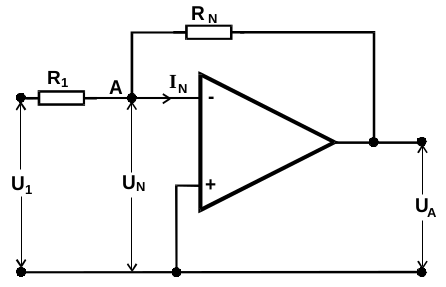
\includegraphics[height=5cm]{ImmerDieseNorweger/gegenkopplung.png}
  \caption{Schematischer Schaltplan für den gegengekoppelten invertierenden Linearverstärker\cite{anleitung}.}
  \label{fig:gegenkopplung}
\end{figure}

Ein Teil der Ausgangsspannung wird zurück auf den invertierenden Eingang gegeben, sodass die Eingangsspannungsdifferenz
und schließlich auch die Ausgangsspannung reduziert wird. Dadurch wird insgesamt ein geringerer Verstärkungsfaktor abhängig von
den eingebauten Widerständen $R_1$ und $R_\text{N}$ erreicht. Mit den Kirchhoffschen Regeln lässt sich für den idealen
Operationsverstärker, für welchen $U_\text{N}$ und $I_\text{N}$ gegen Null gehen, der Verstärkungsfaktor
\begin{align}
  V_\text{id} = \frac{U_\text{A}}{U_\text{1}} = \frac{R_\text{N}}{R_1}
\end{align}
herleiten. Dieser hängt nur von der äußeren Beschaltung des Operationsverstärkers und nicht von ihm selbst ab.
Beim realen Operationsverstärker kann mit der Korrektur, dass die Leerlaufverstärkung endlich ist, der
Verstärkungsfaktor
\begin{align}
  V' \approx \left( \frac1{V} + \frac{R_1}{R_\text{N}} \right)^{-1}
  \label{eqn:leerlaufverst}
\end{align}
hergeleitet werden, wobei $V$ wieder die Leerlaufverstärkung ist. Für den Fall eines großen Widerstandsquotienten
\begin{align}
  \frac{R_1}{R_\text{N}} >> V
\end{align}
geht der reale in den idealen Wert über und der Verstärkungsfaktor ist wieder unabängig von dem Operationsverstärker selbst.
Werden also die Widerstände entsprechend gewählt, so arbeitet der Operationsverstärker stabiler gegen Temperaturschwankungen
und Exemplarstreuungen, sofern die äußere Beschaltung gegenüber diesen stabil ist.
Des Weiteren wird, wie in Abbildung \ref{fig:frequenzband} dargestellt, durch die Gegenkopplungsschaltung ein größeres Frequenzband unverzerrt verstärkt.
Der Vergrößerungsfaktor beträgt dabei
\begin{align}
  g = \frac{V}{V'}.
\end{align}

\begin{figure}
  \centering
  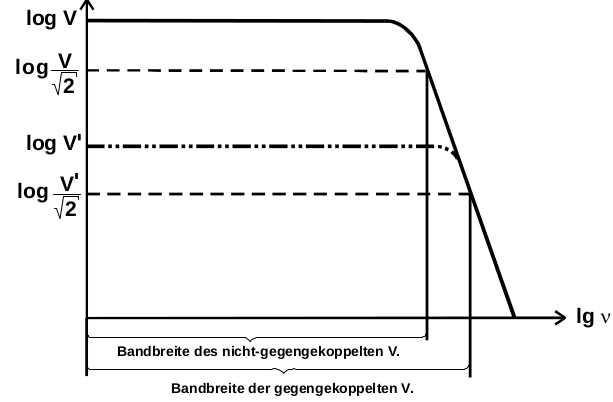
\includegraphics[height=6.5cm]{ImmerDieseNorweger/frequenzband.png}
  \caption{Schematischer Frequenzverlauf beim gegengekoppelten Linearverstärker \cite{anleitung}.}
  \label{fig:frequenzband}
\end{figure}

\subsection{Umkehr-Integrator und Umkehr-Differentiator}

In Abbildung \ref{fig:integrator} ist eine Beschaltung für die Verwendung des Operationsverstärkers
als Umkehr-Integrator abgebildet. Dieser integriert nun eine zeitabhängige Eingangsspannung auf
und skaliert diese mit einem negativen Vorfaktor.
Über die Kirchhoffschen Gesetze kann für den Idealfall einer verschwindenden Differenzeingangsspannung
$U_\text{N} \approx 0$ die Relation
\begin{align}
  U_\text{A}(t) = - \frac1{R C} \int U_1(t) \mathrm{d}t
\end{align}
zwischen Ausgangsspannung $U_\text{A}$ und Eingangsspannung $U_1$ hergeleitet werden.

\begin{figure}
  \centering
  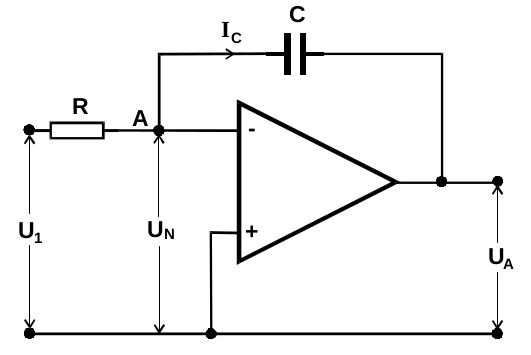
\includegraphics[height=5cm]{ImmerDieseNorweger/integrator.png}
  \caption{Beschaltung für den Operationsverstärker um ihn als Umkehr-Integrator zu verwenden \cite{anleitung}.}
  \label{fig:integrator}
\end{figure}

Für eine sinusförmige Eingangsspannung
\begin{align}
  U_1(t) = U_0 \sin \left( \omega t \right)
  \label{eqn:sinus}
\end{align}
ergibt sich eine Ausgangsspannung mit antiproportionaler Frequenzabhängigkeit
\begin{align}
  U_\text{A}(t) = \frac{U_0}{\omega R C} \cos \left( \omega t \right).
  \label{eqn:int_aus}
\end{align}

Durch Tauschen von Kondensator und Widerstand in der Umkehr-Integrator-Schaltung aus Abbildung \ref{fig:integrator}
wird der Operationsverstärker zum Umkehr-Differentiator umfunktioniert.
Für diese Beschaltung gilt entsprechend
\begin{align}
  U_\text{A}(t) = - RC \frac{\mathrm{d} U_1(t)}{\mathrm{d}t}.
\end{align}
Außerdem ergibt sich für eine sinusförmige Eingangsspannung wie in Gleichung \eqref{eqn:sinus}
eine Ausgangsspannung mit linearer Frequenzabhängigkeit
\begin{align}
  U_\text{A}(t) = - \omega R C U_0 \cos \left( \omega t \right).
  \label{eqn:diff_aus}
\end{align}

\subsection{Schmitt-Trigger}

Anstatt den Operationsverstärker wie beim Linearverstärker mit Hilfe eines Widerstands gegenzukoppeln, kann
er auch mitgekoppelt werden, wie es beim sogenannten Schmitt-Trigger der Fall ist. Dazu wird der Rückkopplungszweig
auf den nicht-invertierenden anstatt auf den invertierenden Eingang
gegeben. Die Funktionsweise ändert sich dabei drastisch, da anstatt einer Abschwächung des Verstärkungsfaktors
eine Verstärkung auftritt. Beim Erreichen bestimmter Schwellenspannungen kippt die Ausgangsspannung dann sofort auf
die Extremalwerte $\pm U_\text{B}$ und der beschaltete Operationsverstärker kann als Komparator verwendet werden.
Die Beschaltung ist in Abbildung \ref{fig:schmitttrigger} skizziert.

\begin{figure}
  \centering
  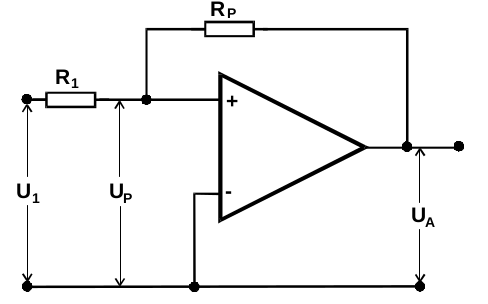
\includegraphics[height=5cm]{ImmerDieseNorweger/schmitttrigger.png}
  \caption{Beschaltung des Operationsverstärkers, damit dieser als Schmitt-Trigger arbeitet \cite{anleitung}.}
  \label{fig:schmitttrigger}
\end{figure}

Die Kippvorgänge finden an den Schwelleneingangsspannungen
\begin{align}
  U_\text{1,krit} = \pm \frac{R_1}{R_\text{p}} U_\text{B}
\end{align}
statt, da genau an diesen Punkten die Eingangsspannung $U_\text{p}$ ihr Vorzeichen
wechselt. Wird also beispielsweise bei einer Ausgangsspannung $-U_\text{B}$ die Eingangsspannnung
auf den positiven Wert $U_\text{1,krit}$ erhöht, so wird $U_\text{p}$ gerade positiv
und verstärkt sich schließlich über den Operationsverstärker mit Rückkopplung selbst,
sodass schlagartig die Ausgangsspannung auf $+U_\text{B}$ kippt. Dieser von der
Vergangenheit der Eingangsspannung abhängende Prozess wird entsprechend auch als Schalthysterese
bezeichnet. Mit Hilfe des Schmitt-Triggers ist es beispielsweise möglich, eine sinusförmige
Eingangsspannung in eine Rechteckspannung mit einer Amplitude von $2 U_\text{B}$ umzuwandeln.

\subsection{Signalgenerator}

Mit Hilfe der in Abbildung \ref{fig:signalgen} aufgezeigten Schaltung können Rechteck- und
Dreieckspannungen erzeugt werden. Der Schmitt-Trigger überführt für sich genommen ein periodisches Eingangssignal,
welches die Schwellenwerte $U_\text{1,krit}$ überschreitet, in eine Rechteckspannung.
Wird die produzierte Rechteckspannung auf den Eingang eines Umkehr-Integrators gegeben, so erzeugt dieser
durch Integrieren eine Dreieckspannung. Da in der vorliegenden Schaltung die Dreieckspannung wiederum direkt mit dem Eingang des
Schmitt-Triggers gekoppelt ist, schwingt das System nach einer externen Anregung von selbst mit Hilfe der Betriebsspannungen $U_\text{B}$.
Es muss also nur ein kurzes periodisches Eingangssignal in das System gebracht werden um den Generator einzuschalten.
Zwischen Schmitt-Trigger-Ausgang und Integrator-Eingang kann entsprechend eine Rechteckspannung und zwischen
Integrator-Ausgang und Schmitt-Trigger-Eingang eine Dreieckspannung abgegriffen werden.
Dabei stellt sich abhängig von den Bauteilen in der Beschaltung eine bestimmte Frequenz und Amplitude bei der
Dreieckspannung ein. Dies wird im Folgenden hergeleitet.

\begin{figure}
  \centering
  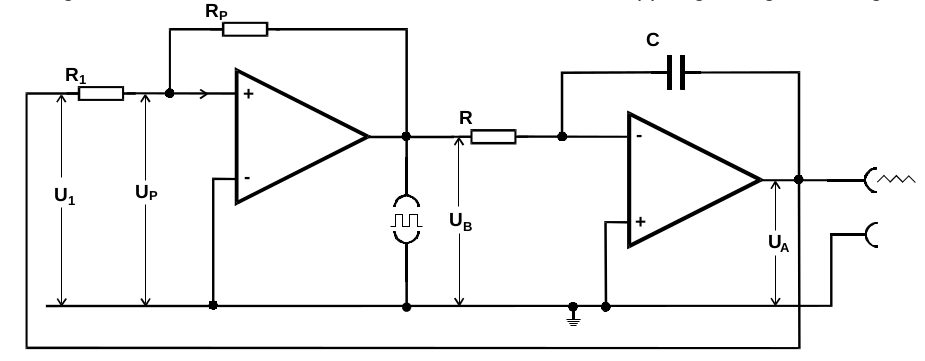
\includegraphics[height=5cm]{ImmerDieseNorweger/signalgenerator.png}
  \caption{Beschaltung zweier Operationsverstärker als Signalgenerator für eine Rechtecks- und Dreieckspannung \cite{anleitung}.}
  \label{fig:signalgen}
\end{figure}

Sobald am Schmitt-Trigger-Ausgang die Spannung $U_\text{B}$ vorliegt, wird diese
durch den Integrator so lange integriert, bis am Integrator-Ausgang bzw. am Schmitt-Trigger-Eingang die Spannung
\begin{align}
  U_\text{1,krit} = - \frac{R_1}{R_\text{p}} U_\text{B}
\end{align}
vorliegt. Für den Startpunkt der Schwingung wird
\begin{align}
  U_\text{A}(0) = 0
\end{align}
gewählt, sodass sich beim ersten Integriervorgang die Abhängigkeit
\begin{align}
  U_\text{A}(t) = -\frac1{RC} U_\text{B} t
\end{align}
ergibt. Jeder vollständige Integriervorgang eines eingehenden Rechteckpulses beschreibt genau eine halbe Periode
der Reckteck- bzw Dreieckspannung. Der erste tatsächliche Integriervorgang nach dem Startzeitpunkt $t=0$ ist jedoch
nur ein halber, da er bei einer Ausgangsspannung von Null startet. Entsprechend beschreibt der erste
tatsächliche Integriervorgang genau ein Viertel der Periode der Ausgangsspannungen.
Nach diesem ersten Integriervorgang kippt die Ausgangsspannung des Schmitt-Triggers, bzw. die Eingangsspannung
des Integrators auf $-U_\text{B}$, sodass der Integrator in Folge eine negative Spannung
aufintegriert. Dies tut er gemäß
\begin{align}
  U_\text{A}(t) = + \frac1{RC} U_\text{B} t - \frac{R_1}{R_\text{p}} U_\text{B}
\end{align}
so lange, bis der Schwellenwert
\begin{align}
  U_\text{1,krit} = + \frac{R_1}{R_\text{p}} U_\text{B}
\end{align}
erreicht ist. Nun beginnt wieder der negative Integriervorgang und sobald wieder eine Ausgangsspannung von Null
erreicht wird, beginnt der gesamte ab dem Zeitpunkt $t=0$ beschriebene Prozess von Neuem. Die Periodendauer entspricht genau der Zeit, in der die Dreieckspannung eine positive
Steigung hat, addiert mit der gleichlangen Zeit, in der die Dreieckspannung eine negative Steigung hat. Bei einem Viertel der Periodendauer
hat die Ausgangsspannung am Integrator, wie bereits oben erwähnt, den
Schwellenwert erreicht, also
\begin{align}
  U_\text{A}\left( \frac{T}{4} \right) = -\frac{T}{4RC} U_\text{B} \stackrel{!}{=} -\frac{R_1}{R_\text{P}} U_\text{B}.
\end{align}
Daraus folgt die Frequenz der Rechteck- sowie der Dreieckspannung
\begin{align}
  \nu = \frac1{T} = \frac{R_\text{p}}{4 R C R_1}.
  \label{eqn:freq_signalgen}
\end{align}
Da die Dreieckspannung genau bei den Umschaltpunkten extremal wird ist ihre Amplitude gleich dem
doppelten Schwellenwert
\begin{align}
  A = \frac{2 R_1}{R_\text{p}} U_\text{B}.
  \label{eqn:ampl_drei}
\end{align}

\subsection{Erzeugung von Sinusschwingungen mit exponentiell variierender Amlitude}

In Abbildung \ref{fig:expsin} ist eine Beschaltung von Operationsverstärkern dargestellt, mit welcher
eine exponentiell zu- bzw. abnehmende Sinusschwingung erzeugt werden kann. Die ersten beiden Operationsverstärker
sind als Umkehr-Integratoren beschaltet, während die Beschaltung des letzten Operationsverstärker ein
Eingangssignal einfach invertiert. Mit Hilfe eines Potentiometers kann außerdem ein Teil der Ausgangsspannung
des Invertierers auf den zweiten Umkehr-Integrator gegeben werden, was genau über die exponentielle Variation
der Sinusamplitude entscheidet. Wird die zurückgegebene Spannung entsprechend auf Null gesetzt, so ist es plausibel,
dass die Eigenschwingung des System ein Sinus ist, da diese Funktion gerade sich selbst ergibt, wenn
zweifach integriert und anschließend ein Vorzeichenwechsel durchgeführt wird.

\begin{figure}
  \centering
  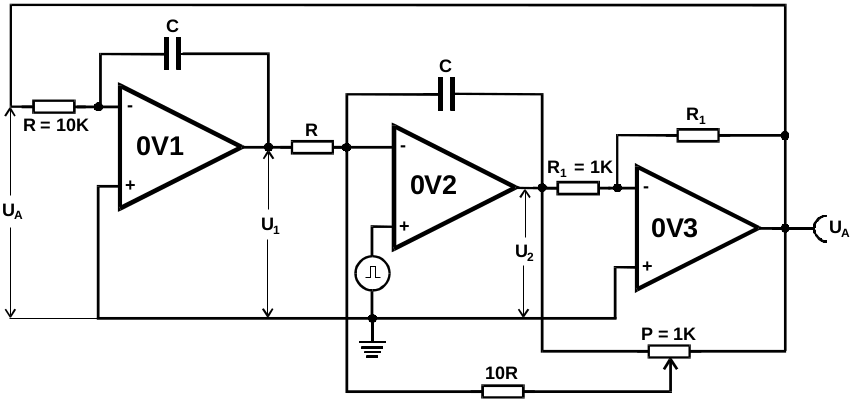
\includegraphics[height=6cm]{ImmerDieseNorweger/expsin.png}
  \caption{Beschaltung dreier Operationsverstärker als Generator von Sinusschwingungen mit exponentiell
  variierenden Amplituden \cite{anleitung}.}
  \label{fig:expsin}
\end{figure}

Für die Eingangs- und Ausgangsspannungen der Integratoren gelten die Beziehungen
\begin{align}
  U_1 = - \frac1{RC} \int U_\text{A} \mathrm{d}t
\end{align}
und
\begin{align}
  U_2 = - \frac1{RC} \int \left(U_\text{A} +\frac{\eta}{10} U_\text{A} \right) \mathrm{d}t,
\end{align}
wobei $\eta$ mit
\begin{align}
  -1 \leq \eta \leq 1
\end{align}
gerade den Bruchteil der Spannung angibt, welcher mittels Potentiometer auf den Eingang des
zweiten Umkehr-Integrators gegeben wird. Aus diesen Gleichungen und der Relation für den Invertierer
\begin{align}
  U_\text{A} = - U_2,
\end{align}
folgt schließlich die Differentialgleichung
\begin{align}
  \ddot{U}_\text{A} - \frac{\eta}{10 RC} \dot{U}_A + \frac1{R^2 C^2} U_A = 0,
\end{align}
welche durch einen Sinus mit exponentiell variierender Amplitude
\begin{align}
  U_\text{A}(t) = U_0 \, \text{exp} \left( \frac{\eta t}{20 RC} \right) \sin \left( \frac{t}{RC} \right)
\end{align}
gelöst wird. Die Frequenz dieser Schwingung beträgt
\begin{align}
  \nu = \frac1{2 \pi R C}.
  \label{eqn:freqexp}
\end{align}
Wie bereits im vorangegangegen Abschnitt plausibel gemacht, ergibt sich eine einfache
Sinusschwingung für $\eta = 0$, wenn also keine Spannung über das Potentiometer auf den zweiten
Operationsverstärkereingang zurückgegeben wird. Für $\eta < 0$ ergibt sich eine gedämpfte, während sich für
$\eta > 0$ eine entdämpfte Sinusschwingung mit der Abkling- bzw. Zunahmedauer
\begin{align}
  \tau = \frac{20 RC}{\lvert\eta\rvert}
  \label{eqn:tauentdämpft}
\end{align}
ergibt.
